\section{Testing}

\subsection{Search Domains Analysis}

After performing the unit testing, the library still has to be proven reliable
and fast in different search domains. To do so, we will use these domains:

\begin{itemize}
\item \textbf{N-Queens}: This problem consists in placing $n$ queens in a $n
  \times n$ chess board so that no two queens are in the same row, column or
  diagonal: that is, placing all the queens without two queens threatening each
  other. This problem is provided in the library under the module
  \texttt{Search.[...].ToyProblem.NQueens}, and this is the implementation that will
  be used to test the performance.
\item \textbf{8-Puzzle}: This problem uses a $3 \times 3$ board that contains 8
  numerated tiles and a blank space. The tiles can be slide around the board if
  they are next to the blank space, and the purpose of the puzzle is to end up
  with a sorted board. This problem is provided in the library under the module
  \texttt{Search.[...].ToyProblem.EightPuzzle}.
\item \textbf{Moving AI Maps}: This problem depends receives a map and two
  coordinates, and the agent generated tries to find a path that goes from one
  point to the other. Depending on the algorithm, this path will be the easier
  to find or the shortest. The map file is expected to be in the format
  provided by \cite{movingai-benchmarks}. This is the most demanding problem of
  all to be tested, as well as the most versatile. A parser for this kind of
  maps is included in \texttt{Search.[...].ToyProblem.MapParser}.
\end{itemize}

In each problem, a different capability of the library is tested, and it will
be explained in depth in each of the domains subsections. To perform these
tests, the included tools with the library will be used to perform all
measurements.\\

\subsubsection{Results \& Performance in N-Queens}

The implementation for the N-Queens problem included with the library uses as
operators the fact of adding a queen to a new column in all possible positions.
That way, the approach followed to solve this problem is a brute-force
approach, which is ideal to study all the uninformed algorithms. On the other
hand, there is no heuristic available for this approach, so the informed set of
algorithms cannot be tested in this domain. For the same reason, no correctness
of the solution has to be considered: if the solution is found is because it is
valid. That makes the evaluation simpler to understand for this case.\\

\begin{figure}[htbp!]
  \centering
  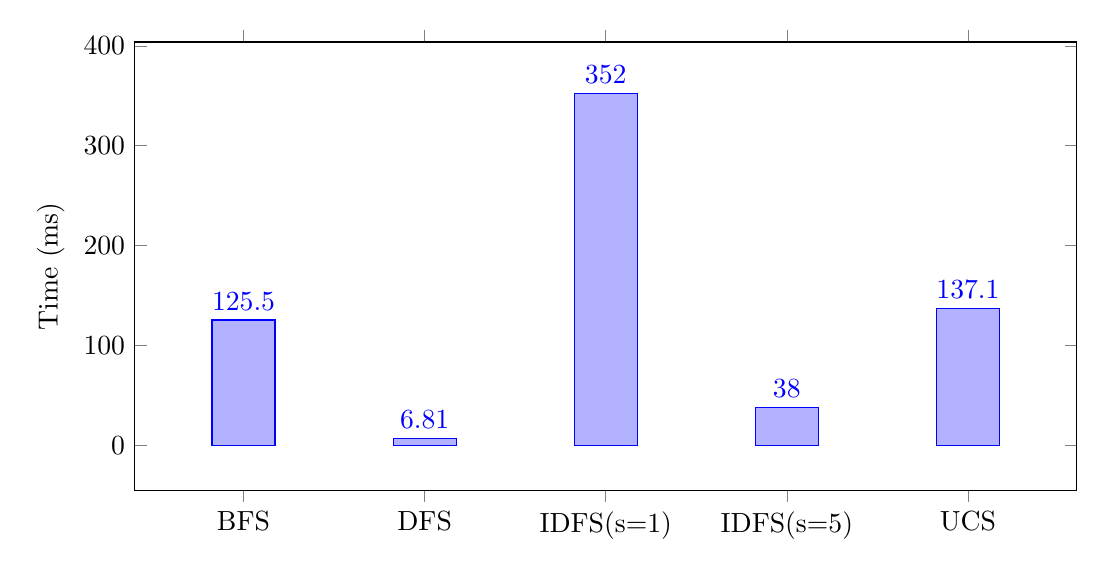
\begin{tikzpicture}
    \begin{axis}[
      ybar,
      enlargelimits=0.15,
      x = 2.3cm,
      bar width = 0.8cm,
      legend style={at={(0.5,-0.15)},
        anchor=north,legend columns=-1},
      ylabel={Time (ms)},
      symbolic x coords={BFS,DFS,IDFS(s=1),IDFS(s=5),UCS},
      xtick=data,
      nodes near coords,
      nodes near coords align={vertical},
      ]
      \addplot coordinates {
        (BFS,125.5)
        (DFS,6.806)
        (IDFS(s=1),352.0)
        (IDFS(s=5),38.0)
        (UCS,137.1)
      };
      % \legend{}
    \end{axis}
  \end{tikzpicture}
  \caption{Time per pure uninformed algorithm in 8-Queens}
  \label{nq:time}
\end{figure}


\subsubsection{Results \& Performance in 8-Puzzle}

\subsubsection{Results \& Performance in Moving AI Maps}


\subsection{Unit \& Integration Testing}

Thanks to the Cabal packaging tool, it is easy to include a test suite in the
library, that can be run automatically. The chosen way to test the functions of
the library was to create a \texttt{Test} folder, in which replicate the
structure of the library modules. In each of this new modules there should be
all the tests for the functions included in them. Since the design of the
library functions are incremental, these small specifications can be both unit
tests (for instance, to check if \texttt{Search.DataStructure.Queue} correctly
adds a node) or integration tests (if a queue and a general search can be
combined correctly to work as a Breadth-First Search). To perform the latter
tests, we will use small examples of each of the search domains that have been
included in the library as toy problems, to test the correctness of the results
returned.\\

To perform this task, the easiest way is to use the \texttt{hspec} package,
that offers all the necessary functions to perform the testing of the modules,
plus a function to discover and run all necessary \texttt{Spec} files when
asking the library to be tested. That way, we can just create new test modules
and they will be automatically discovered. To run the tests it is only
necessary to build the library along with the tests (\texttt{cabal build
  --enable-tests}) and then run \texttt{cabal test}. This convenient access to
the tests is the cornerstone for the Continuous Integration of the library,
that will be specified later on the document.\\

Running this command in the version for this thesis (\texttt{0.2.0.0}) runs a
total of 156 different examples (both unit and integration tests) in
$\sim 2.6581$ seconds with 0 failures. The output presents the name of each of
the modules being tested, along with a description of each of the tests and a
mark in case there was a failure in such example. The complete set of tests can
be found in the path \texttt{src/Test/} of the library code.\\


\subsection{Profiling}

As seen in previous sections, the library has an overall good performance, but
under certain conditions the it becomes drastically slower. However, it is hard
to say what is exactly happening: due to the side-effects isolation, there is
no easy way to use print-debugging or to time different functions of the code
to see what is exactly going on. At this level of abstraction, what the
computer is doing in the bad performances is, indeed, completely hidden from
us.\\

However, the language provides certain tools to profile code if it is indeed
necessary to spot a problem. The main tool for profiling is using the
\texttt{+RTS} interface, that will be detailed next. After explaining the
process of creating a working environment to profile the project, we will
undergo several experiments to find the hot spots in the project and follow a
procedure to fix it.\\

\subsubsection{Creating the \texttt{profiling} executable}

To effectively profile code in Haskell, it is needed to make use of an
interface to the Runtime System (RTS). This system, which is not usually
intended to be directly queued, is the one in charge of a lot of Haskell's nuts
and bolts: RTS includes a storage manager, a scheduler and a profiler, among
other necessary runtime services that work as a middle system between the user
code and the compiled Haskell code \cite{ghc}.\\

To effectively profile the code, it is necessary to use both compilation and
runtime flags. This is usually easy to manage with single files, but a project
like this can become really hard to compile with a simple \texttt{ghc} command
outside of a packaging tool like Cabal or Stack. Plus, the library needs to
install the profile version of the dependencies, so simply compiling by hand
may not be enough to successfully profile the code.\\

The best solution available for a project this size is to create a Cabal
executable that will gather all the options, and enables for an easy access to
the profiling of the library. To create this executable, we need to add the
Listing \ref{prof-cabal} to the file \texttt{agis.cabal} in the root of the
project.\\

\begin{lstlisting}[style=haskell, label=prof-cabal, caption=
Setup for the \texttt{profiling} executable in the Cabal file]
-- Library profiling executable
executable profiling

  hs-source-dirs:      src/Search/Pure
           
  main-is:             Profiling.hs
  
  ghc-options:         -O2
                       -threaded
                       "-with-rtsopts=-N -p -s -h -i0.1"

  build-depends:       [...]

  default-language:    Haskell2010
\end{lstlisting}

This configuration creates a new executable called \texttt{profiling}, that
will call the file \texttt{Profiling.hs} in the directory
\texttt{search/Search/Pure}. This file will simply contain a main method
calling the code to be tested, which will be the main method for the Moving AI
maps. For this executable to created, we pass several options to the compiler:
to be compiled with level 2 optimizations (\texttt{-O2}) and using the
concurrent abstractions (\texttt{-threaded}), as well as to include all the
necessary runtime options (\texttt{-with-rtsopts}):

\begin{itemize}
\item \texttt{-N} sets the number of available processors to the number of
  processors of the system.
\item \texttt{-p} generates the profiling report.
\item \texttt{-s} includes garbage collection in the report.
\item \texttt{-h} includes memory usage in the report.
\item \texttt{-i} sets the profiler frequency to 0.1 seconds.  
\end{itemize}

Running \texttt{cabal build} will compile the project (and install all the
necessary profiling version of the dependencies) and generate the executable.
To run it, it is only necessary to run \texttt{cabal run profiling}. This
shortcut is much more robust and simple than to input the compiler flags every
time. Once run, it outputs a brief description of the profiling in the memory
and generates a comprehensive report (a \texttt{.prof} file) where the runtime
statistics are detailed. Now that the environment is set, we can proceed to
profile the code searching for the hot spots in the library.


\subsubsection{Finding the hot spots of the library}



\subsubsection{Tuning the garbage collection}

After running the profiling experiments in the code, we have found that
problems with a fast growing queue generate a problematic space overhead, that
is translated to big garbage collection pauses that make execution slow. The
cost centers reveal that the space allocation happen most of all in the
\texttt{DataStructure} methods for adding nodes, so let us keep researching how
to fix this issue. To generate a lot of nodes in the open list, we will use a
bad heuristic in the problem \texttt{Warcraft}, to get a solution with these
statistics (obtained with the \texttt{Search.Monadic} library):

\begin{itemize}
 \item Number of expanded nodes: 378790
 \item Number of enqueued nodes: 734887
 \item Maximum length of the queue: 356099
\end{itemize}

Just to obtain a plan length of 19. This big size for the open list will
trigger the garbage collection problem and let us study it better. The mean
execution time for this problem in the original implementation is 11.573
seconds; which may seen acceptable but increases rapidly with the plan length
(a new node can add 8-10 seconds to this execution time). This small size is
found to be the \\

Now, to experience the impact of the garbage collector settings we will use a
tool called \texttt{ghc-gc-tune} \cite{ghc-gc-tune}. This tool will allow us to
brute force the garbage collector options and get a general insight of the
behavior of the program under different settings. This will let us see if the
problem is originated by the garbage collector being too intrusive or if there
is a reason intrinsic to the implementation of the program. The tool needs to
be fed an executable with the RTS options open for modification, we need to
design a new executable:\\

\begin{lstlisting}[style=haskell, label=gc-cabal, caption=
Setup for the \texttt{gc-tuning} executable in the Cabal file]
-- Library garbage collection tuning executable
executable gc-tuning

  hs-source-dirs:      src/Search/Pure
           
  main-is:             Profiling.hs
  
  ghc-options:         -O2
                       -threaded
                       -rtsopts

  build-depends:       [...]

  default-language:    Haskell2010
\end{lstlisting}

This executable uses the file \texttt{Search/Pure/Profiling.hs}, as well as the
previous executable used, but this time the RTS options are left open instead
of providing some. This is necessary because the access to the RTS is
considered a vulnerability and it is disabled for all packages compiled by
default. Once we have linked with \texttt{-rtsopts}, we can run the tool. After
a long execution trace, the following results are returned:\\

\begin{lstlisting}
Best settings for Running time:
5.43s:  +RTS -A16384 -H536870912
5.49s:  +RTS -A536870912 -H1073741824
5.52s:  +RTS -A268435456 -H536870912
5.68s:  +RTS -A4194304 -H536870912
5.68s:  +RTS -A268435456 -H1073741824
\end{lstlisting}

Under some garbage collection settings, it is possible to improve the total
execution time in a 50\%. Without having to refactor the code, it is possible
to cut in half the time just by setting some options in the garbage collection.
Although this results are good, let us not be over-optimistic: by tuning this
executable we may be making the execution options specific to the problem that
is being used, instead of obtaining a general improvement. Over-fitting the
library to this concrete example is at risk.\\

\begin{figure}[ht]
\centering
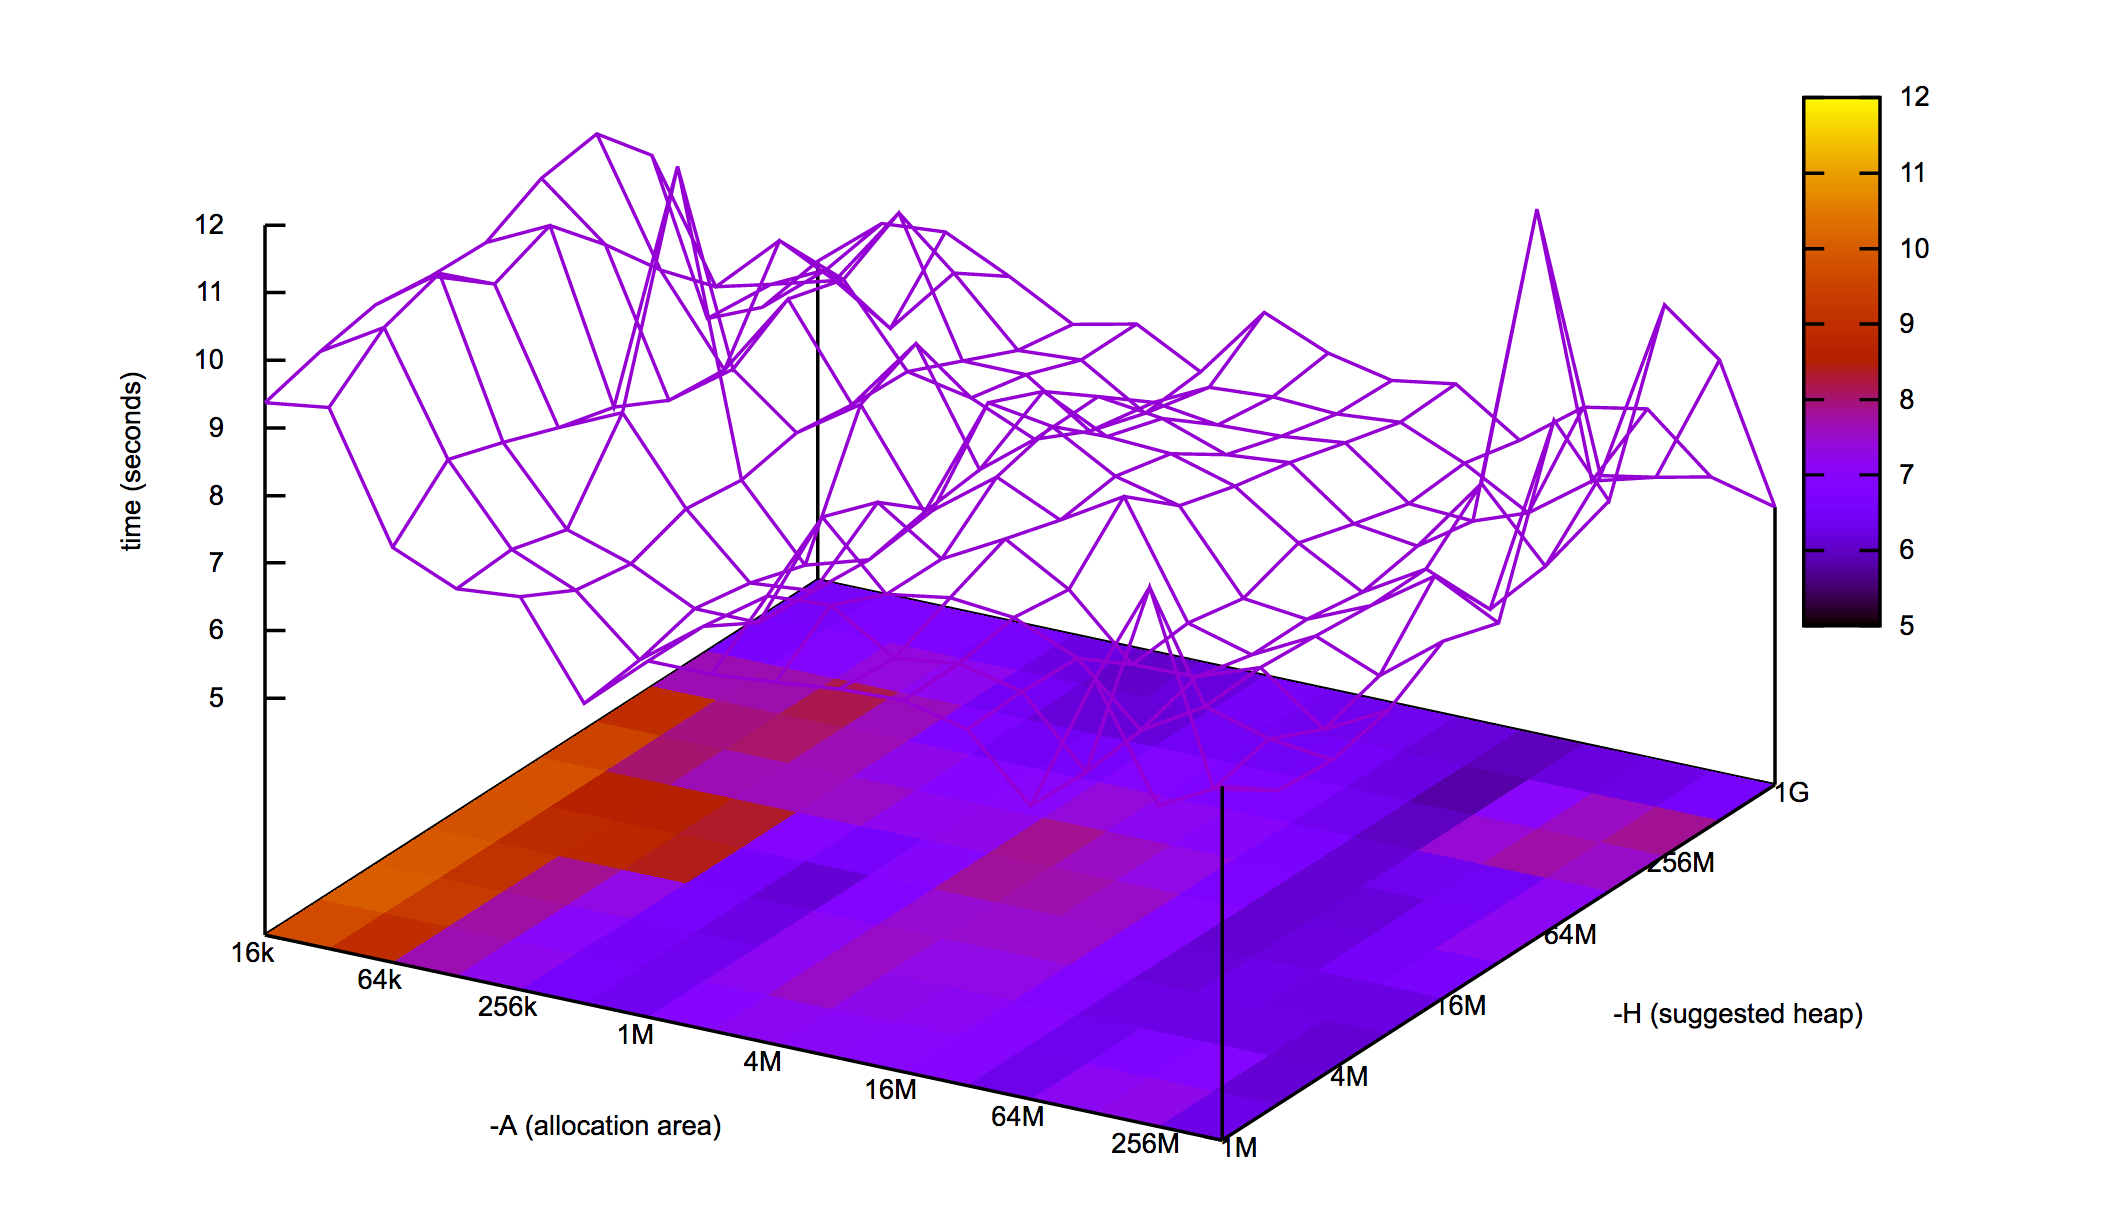
\includegraphics[width=\textwidth]{img/gc-tuning.png}
\caption{Garbage collection flags compared to execution time.}
\label{gc-tuning}
\end{figure}

To check if that is indeed the case, we can take a look at the general spectrum
of results generated by the tool (Figure \ref{gc-tuning}). In there, we can see
that the garbage collection settings are of great importance for the library:
in the plane that represents the different execution times, a flat shape would
indicate that there is not much influence done by the garbage collection. In
the plot we can see the opposite: a strenuous surface that represents the time
the execution expends on garbage collection, on how a difference in the
allocation space or heap available can increase up to a 40\% the total
computation time. In the results, there is an expected peak when the garbage
collection settings force the use of low memory, and its counterpart when the
settings are high. Although it may be tempting to offer the program the highest
memory flags to be sure of low execution times, this may be counter-productive
in lower-memory systems and parallel applications.\\

To check if the flags are, indeed, being a benefit for a general number of
nodes expanded, the Figure XXXXX shows a side by side plot of different plan
lengths in the same problem, with and without using any garbage collection
flags.

%%% TODO:

\subsubsection{Profiling different \texttt{PriorityQueue} implementations}


Now that we have discarded a substantial improvement by tuning with flags the
garbage collection, it's time to analyze the \texttt{PriorityQueue}
implementation and try to find if there is something to be improved in the
code. The code implements the priority queue over a package called
\texttt{heap}, which promises to deliver ``\textit{a flexible implementation of
  min-, max-, min-priority, max-priority and custom-priority heaps based on the
  leftist-heaps from Chris Okasaki's book Purely Functional Data Structures}''
\cite{okasaki-1999-purely}, which was exactly what was desired when
implementing the library (to follow the explanations in the literature).
However, this package may not be as suitable as thought for our purposes or it
may be a misuse of it. Running the \texttt{profiling} executable of the library
in this problem outputs, we can see these results (please bear in mind the
profiling overhead, stated as \texttt{PROF} time):\\

\begin{lstlisting}
> cabal run profiling
   4,452,597,512 bytes allocated in the heap
   5,673,545,840 bytes copied during GC
     234,847,840 bytes maximum residency (45 sample(s))
       1,616,992 bytes maximum slop
             472 MB total memory in use (0 MB lost due to fragmentation)

                                     Tot time (elapsed)  Avg pause  Max pause
  Gen  0      8573 colls,     0 par    1.030s   1.050s     0.0001s    0.0004s
  Gen  1        45 colls,     0 par    7.107s   7.359s     0.1635s    0.3832s

  TASKS: 4 (1 bound, 3 peak workers (3 total), using -N1)

  SPARKS: 0 (0 converted, 0 overflowed, 0 dud, 0 GC'd, 0 fizzled)

  INIT    time    0.001s  (  0.010s elapsed)
  MUT     time    3.333s  (  5.247s elapsed)
  GC      time    6.249s  (  6.495s elapsed)
  RP      time    0.000s  (  0.000s elapsed)
  PROF    time    1.888s  (  1.914s elapsed)
  EXIT    time    0.003s  (  0.046s elapsed)
  Total   time   11.475s  ( 11.797s elapsed)

  Alloc rate    1,335,764,960 bytes per MUT second

  Productivity  29.1% of total user, 28.6% of total elapsed
\end{lstlisting}


We can see how the profiler returns that only a 29.1\% of the time has been
spent in actual search computations, while more than half of the execution time
(54.5\%) has been spent in garbage collection. To check if this space leak is
caused by our implementation or by the library used to implement the priority
queue, we can experiment with different methods.\\

We can run the same problem using the implementation with the \texttt{psqueues}
(and more accurately the \texttt{Data.IntPSQ} module), an alternative library
that offers an implementation of a higher level than our original \texttt{heap}
package. The results are as follow:\\


\begin{lstlisting}
> cabal run profiling
   4,867,074,880 bytes allocated in the heap
   4,823,508,568 bytes copied during GC
     183,851,592 bytes maximum residency (46 sample(s))
       1,405,912 bytes maximum slop
             373 MB total memory in use (0 MB lost due to fragmentation)

                                     Tot time (elapsed)  Avg pause  Max pause
  Gen  0      9345 colls,     0 par    0.992s   1.017s     0.0001s    0.0018s
  Gen  1        46 colls,     0 par    5.654s   5.849s     0.1271s    0.2936s

  TASKS: 4 (1 bound, 3 peak workers (3 total), using -N1)

  SPARKS: 0 (0 converted, 0 overflowed, 0 dud, 0 GC'd, 0 fizzled)

  INIT    time    0.001s  (  0.012s elapsed)
  MUT     time    3.508s  (  4.884s elapsed)
  GC      time    5.292s  (  5.498s elapsed)
  RP      time    0.000s  (  0.000s elapsed)
  PROF    time    1.354s  (  1.367s elapsed)
  EXIT    time    0.003s  (  0.037s elapsed)
  Total   time   10.159s  ( 10.431s elapsed)

  Alloc rate    1,387,545,376 bytes per MUT second

  Productivity  34.6% of total user, 34.1% of total elapsed
\end{lstlisting}


There, it can be seen that the garbage collection time has been reduced by a
second, but it is still a marginal improvement. Therefore, maybe a different
approach is needed: If we take a close look to the \texttt{addList} method, the
main cost center of this problem, we can see that we have two main options to
implement it: the first of them is to create a new \texttt{MinPrioHeap} and use
the library function \texttt{union} to merge both of them inside the new
structure. The code is shown in the listing \ref{addlist:union}.\\

\begin{lstlisting}[style=haskell, caption= \texttt{addList} using
  \texttt{union}, label=addlist:union]
addList xs (PriorityQueue h f) = PriorityQueue (union h xs') f
  where xs' = fromList $ map (\n -> (f n, n)) xs
\end{lstlisting}

Although the language should manage the memory correctly, maybe this is not the
best way of managing this operation. As a possible solution, we can try to
force the reutilization of the old structure by adding the nodes using a strict
fold over the \texttt{MinPrioHeap}. This implementation is shown in the listing
\ref{addlist:fold}.\\

\begin{lstlisting}[style=haskell, caption= \texttt{addList} using
  \texttt{fold'}, label=addlist:fold]
addList xs (PriorityQueue h f) = PriorityQueue (foldl' insertNode h xs) f
  where insertNode acc x = insert (f x, x) acc
\end{lstlisting}

To check the performance of all possibilities, the profiling problem stated at
the beginning of this subsection has been run using all combination of
implementations and library, and the full results of performance are found in
the chart shown in the figure \ref{chart-libraries}.\\

\begin{figure}[ht]
  \centering
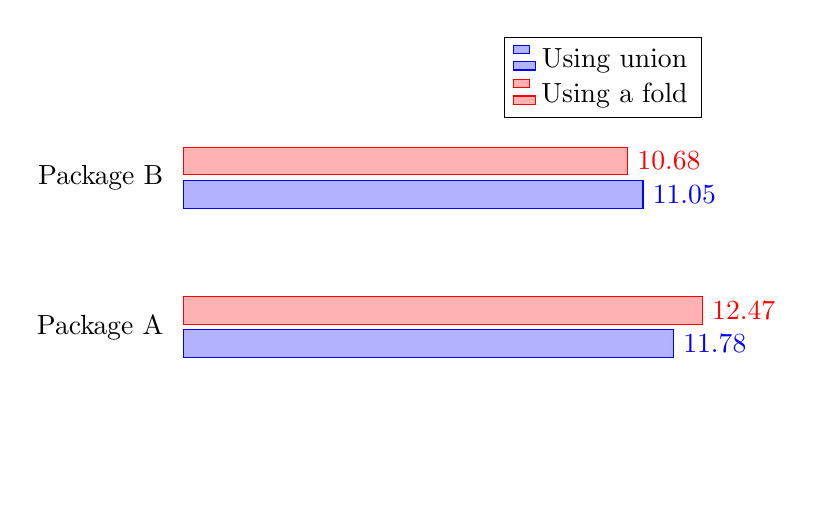
\begin{tikzpicture}
  \begin{axis}[
    xbar,
    y axis line style = { opacity = 0 },
    axis x line       = none,
    % width = 8cm, height = 4cm,
    ytick = data,
    xmin=0,
    tickwidth         = 0pt,
    enlarge y limits  = 1,
    enlarge x limits  = 0.02,
    symbolic y coords = {Package A,Package B},
    nodes near coords,
  ]
  \addplot coordinates { (11.779,Package A) (11.046,Package B) };
  \addplot coordinates { (12.473,Package A) (10.677,Package B) };
  \legend{Using union, Using a fold}
  \end{axis}
\end{tikzpicture}
\vspace{-1cm}
\caption{Comparing Package A (\texttt{heap}) and Package B
  (\texttt{psqueues}).}
\label{chart-libraries}
\end{figure}

It can be seen how the performances are very similar to each other: no matter
which library or what implementation we use. We can then conclude that the
problem is intrinsic to the memory management performed by the RTS interface in
Haskell, or by how the compiler is turning the high-level declarations into
machine code.\\

Nonetheless, taking into account the knowledge that has been obtained by
profiling the data structure, the most intuitive and possible reason for this
space leak is that in Haskell, all data in immutable, and by adding the nodes
to the queue a complete new queue is being generated, allocating a new copy of
it and forcing the garbage collector to claim the old queue's space. Although
this is the natural behavior expected from the language, there are workarounds
to make a data structure mutable, but it has been impossible to find an
implementation that allows for a low complexity insertion and extraction of
nodes in a sorted heap and that is mutable. Implementing such data structure in
Haskell is not an easy task, and it is considered to be out of the scope of
this thesis.\\

\newpage

%%% Local Variables:
%%% TeX-master: "tfg"
%%% End: